\chapter{Fundamentação Teórica}
\label{cap:fundamentacao-teorica}

Sommerville (2007) definiu engenharia de software como uma disciplina da engenharia que cuida de todos os aspectos da produção de software, desde a especificação do sistema até a sua manutenção, depois que ele entra em operação. 
A engenharia é constituída de processos de software, que são conjuntos de atividades e resultados para se produzir um software. Existem quatro atividades fundamentais, são elas: 
Especificação de Software: o software a ser desenvolvido e as restrições para sua operação são definidos. 
Desenvolvimento de Software: o software deve ser feito atendendo suas especificações. 
Validação de Software: o software tem de ser validado para garantir que está em cima do que o cliente deseja. 
Evolução do Software: o software sofre modificações para atender as necessidades do cliente. 
No desenvolvimento de software, o principal objetivo é a criação de sistemas que atendam às necessidades dos clientes e usuários, ou seja, uma correta especificação dos requisitos se torna essencial para que o desenvolvimento tenha sucesso. Uma forma de entender melhor esses requisitos é dividindo-os em: Requisitos Funcionais e Requisitos Não-Funcionais, Vasconcelos, Rouiller, Machado e Medeiros (2006). 
Os Requisitos Funcionais definem as funções que componentes do sistema ou sistemas devem executar. 
Os Requisitos Não-Funcionais incluem limitações no produto, como por exemplo: desempenho, confiabilidade, segurança e limitações no desenvolvimento, como custos e tempo, componentes a serem reutilizados, entre outros.

\section{Desenvolvimento Mobile}
\label{sec:desenvolvimento-mobile}

\lipsum[10]

	\begin{figure}[h!]
		\centering
		\Caption{\label{fig:exemplo-1} Lorem ipsum dolor sit amet, consectetur adipiscing elit. Suspendisse commodo lectus et augue elementum varius.}	
		\UECEfig{}{
			\fbox{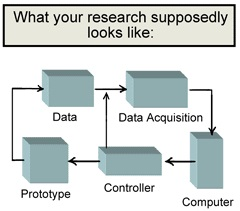
\includegraphics[width=8cm]{figuras/figura-1}}
		}{
			\Fonte{Elaborado pelo autor}
		}	
	\end{figure}
	
\lipsum[11]


\section{Scrum}
\label{sec:scrum}

Scrum é uma metodologia ágil para gestão e planejamento de projetos de softwares e sua base fundamental pode ser bem descrita na imagem abaixo.

	\begin{figure}[h!]
		\centering
		\Caption{\label{fig:exemplo-2} Maecenas luctus augue odio, sed tincidunt nunc posuere nec}	
		\UECEfig{}{
			\fbox{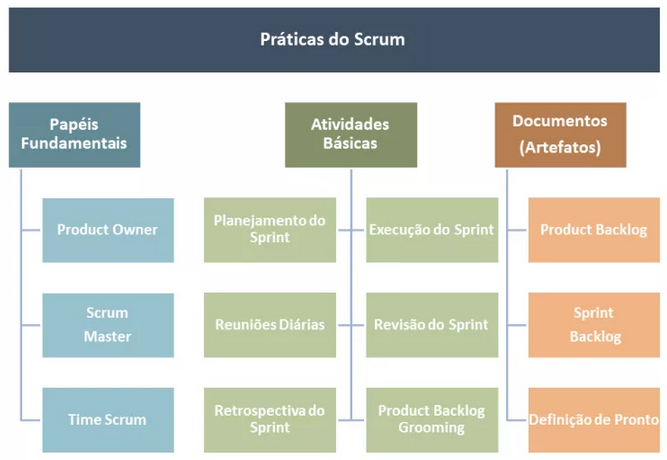
\includegraphics[width=10cm]{figuras/PraticaScrum}}
		}{
			\Fonte{Elaborado pelo autor}			
		}	
	\end{figure}

Cada equipe de Scrum, geralmente, possuem 3 papeis:
\begin{alineascomponto}
	\item ProductOwner
É responsável por decidir os recursos e funcionalidades utilizadas no projeto é também sua responsabilidade manter clareza no objetivo do projeto, para que haja uma melhor interação o ProductOwner geralmente colabora com o ScrumMaster.

	\item ScrumMaster
É de sua responsabilidade ajudar todos envolvidos a entender os valores, princípios e práticas do Scrum. Também fica responsável por melhorias no uso do Scrum e está sempre orientando para que não haja a perda de foco. 

	\item Development Team
São todos da equipe responsáveis pelo desenvolvimento em si do software, possuem papeis como: arquiteto, testador, programador e etc.. Para esta equipe é recomendável que se organizem para determinar a melhor maneira de realizar o trabalho.

	\end{alineascomponto}
	
A imagem abaixo representa o processo de interação das atividades

	\begin{figure}[h!]
		\centering
		\Caption{\label{fig:exemplo-3} Ut posuere, ex quis sagittis auctor, magna massa euismod felis}	
		\UECEfig{}{
			\fbox{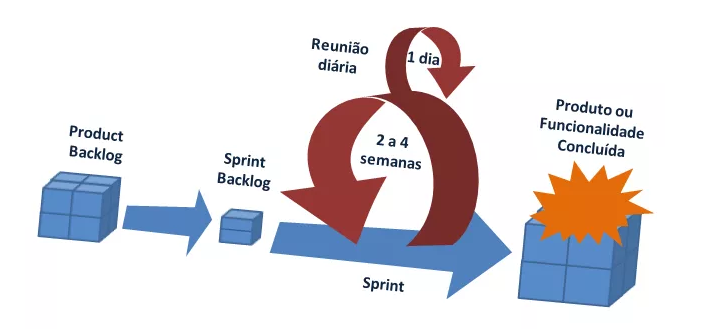
\includegraphics[width=10cm]{figuras/InteracaoScrum}}
		}{
		\Fonte{Elaborado pelo autor}			
	}	
	\end{figure}
	
O ProductOwner tem a visão final do produto, representado na figura como grande cubo. Este cubo é "divido" em vários outros cubos pequenos, este chamado de ProductBacklog.
O ProductBacklog pode ser descrito, em uma forma simplificada, como pequenas etapas/objetivos para se chegar ao produto final.
Para planejar a prioridade dos Backlogse também quando e quanto tempo durará seu desenvolvimento, é utilizado o Sprint.
O Sprint tem duração mediana de 2 a 4 semanas, mas é também flexível dependendo do tempo desenvolvimento final estimado no começo do planejamento.

	\begin{figure}[h!]
		\centering
		\Caption{\label{fig:exemplo-4} Ut posuere, ex quis sagittis auctor, magna massa euismod felis}	
		\UECEfig{}{
			\fbox{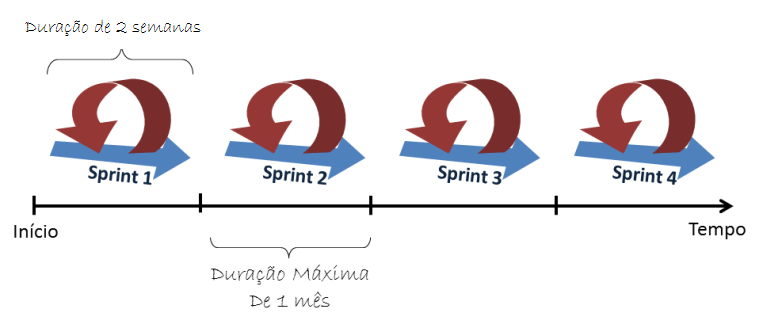
\includegraphics[width=10cm]{figuras/DuracaoSprint}}
		}{
		\Fonte{Elaborado pelo autor}			
	}
	\end{figure}



\section{Controle de Versão}
\label{sec:Controle-de-Versão}